
% This LaTeX was auto-generated from MATLAB code.
% To make changes, update the MATLAB code and republish this document.

\documentclass{article}
\usepackage{graphicx}
\usepackage{color}

\sloppy
\definecolor{lightgray}{gray}{0.5}
\setlength{\parindent}{0pt}

\begin{document}

    
    \begin{verbatim}
%Q1(e)
% Explanation : For dt = 1, we see unexpected behaviour as value of T
% reaches above 25 C. For dt = 0.5, curve is not smooth as that seen for dt
% = 0.1 and dt = 0.5. For dt = 0.1 and dt = 0.05 curve almost coincides
% hence either of the value of dt is suitable. But for dt = 0.1 number of computations are less %hence it is preferable.
close all;
clear all;
Tm = 25;
k = 0.000370834 * 3600;
dt1 = [1, 0.5, 0.1, 0.05];
total = 6;
set(gca,'fontsize',13)
hold on
for j = 1 : 4
    dt = dt1(j);
    iter = (total - 1) / dt + 1;
    T = zeros(iter, 1);
    T(1) = 6;
    t = zeros(iter, 1);
    for i = 2 : iter
        T(i) = T(i - 1) - dt * (k * (T(i - 1) - Tm));
        t(i) = t(i - 1) + dt;
    end
    plot(t, T,'lineWidth',1.5)
    hold on
end
legend(strcat('dt=',num2str(1)), strcat('dt=',num2str(0.5)), strcat('dt=',num2str(0.1)), strcat('dt=',num2str(0.05)));
title('Comparison of different values of dt');
xlabel('Time (in hours)');
ylabel('Temperature (in degree celcius)');
\end{verbatim}

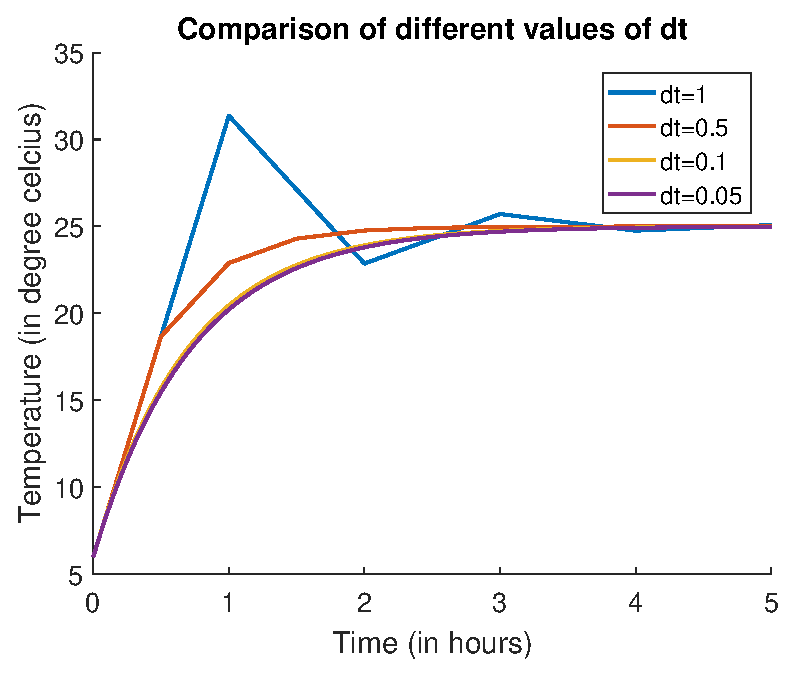
\includegraphics [width=4in]{q1e_01.eps}



\end{document}
    
